\documentclass[sigconf,anonymous,review]{acmart}

%% ---------------------------------------------------------------
%% Compile with pdfLaTeX (Overleaf default). acmart then loads the
%% official ACM fonts (Linux Libertine + newtxmath).
\makeatletter
\@ifundefined{mathbb}{\usepackage{amsfonts}}{}
\makeatother
%% ---------------------------------------------------------------

%% Allow slightly looser lines instead of overfull boxes.
\setlength{\emergencystretch}{1.5em}
\usepackage{booktabs}
\usepackage{multirow}
\usepackage{makecell}
\usepackage{graphicx}

\setcopyright{none}
\copyrightyear{2027}
\acmYear{2027}
\acmConference[WWW '27]{The ACM Web Conference 2027}{May 10--14, 2027}{Dublin, Ireland}
\acmBooktitle{Proceedings of The ACM Web Conference 2027 (WWW '27)}
\acmDOI{}
\acmISBN{}
\settopmatter{printacmref=true}


%% ---------------------------------------------------------------
%% Review marks (yellow background, red bold).
%%   \tbd{...}  placeholder that MUST be filled before submission;
%%              always highlighted.
%%   \ph        numeric placeholder (prints X.XX); MUST be replaced.
%%   \ai{...}   wording flagged for human review; set \reviewmarksfalse
%%              to print it as normal text once reviewed.
%% Before submission: searching the project for "\tbd{" and "\ph"
%% must return only these definitions.
\usepackage{xcolor}
\newif\ifreviewmarks
\reviewmarkstrue
\ExplSyntaxOn
\seq_new:N \l__rev_words_seq
\bool_new:N \l__rev_first_bool
\NewDocumentCommand{\revhl}{m}
  {
    \group_begin:
    \setlength{\fboxsep}{0.6pt}
    \color{red}\bfseries
    \seq_set_split:Nnn \l__rev_words_seq {~} {#1}
    \bool_set_true:N \l__rev_first_bool
    \seq_map_inline:Nn \l__rev_words_seq
      {
        \bool_if:NTF \l__rev_first_bool
          { \bool_set_false:N \l__rev_first_bool }
          { \colorbox{yellow}{\strut\hspace{0.25em}}\hskip 0pt plus 0.15em\relax }
        \colorbox{yellow}{\strut ##1}
      }
    \group_end:
  }
\ExplSyntaxOff
\newcommand{\tbd}[1]{\revhl{#1}}
\newcommand{\ph}{\revhl{X.XX}}
\newcommand{\ai}[1]{\ifreviewmarks\revhl{#1}\else#1\fi}
%% ---------------------------------------------------------------

\newcommand{\method}{Omni-Aware}
\newcommand{\Uomni}{U_{\mathrm{omni}}}
\newcommand{\hgrd}{\mathcal{H}_{\mathrm{grd}}}
\newcommand{\hpred}{\mathcal{H}_{\mathrm{pred}}}
\newcommand{\taub}{\tau_{\mathrm{bias}}}
\newcommand{\Mbias}{M_{\mathrm{bias}}}
\newcommand{\tans}{t_{\mathrm{ans}}}
\newcommand{\tend}{t_{\mathrm{end}}}
\newcommand{\webimg}{WebQA-img}

\begin{document}


\title[Omni-Aware: Latent-Space Evidence Control]{Omni-Aware: Latent-Space Evidence Control for Multimodal Web Answering}

\author{Anonymous Author(s)}
\affiliation{\institution{Anonymous Institution}\country{}}

\begin{abstract}
Web retrieval-augmented generation (Web RAG) answers questions from Web evidence that may lie in text passages, images, tables, or video frames. Existing multimodal RAG systems decide when and where to retrieve with format-specific uncertainty signals and rules, making these decisions hard to coordinate across formats. They also leave the influence of the retrieved evidence to position-sensitive attention, so reordering the same evidence can change the answer. We propose \method{}, a training-free controller that operates in the latent space of evidence spans, the token spans that encoded evidence occupies in the decoder input. A single zero-bias prefill over the evidence spans, those of the supplied context or, at cold start, of a probe round of retrieved chunks, yields all three control decisions: one uncertainty score from predictive entropy and the dispersion of evidence attention decides whether to retrieve, the share and dispersion of that attention across modalities decide which modality to search, and the same score gates Evidence Attention Bias (EAB), which adds a relevance-weighted bias to the attention logits of retrieved chunks on every row that predicts an answer token. The controller trains no router or classifier, samples no extra generations, and changes neither the input nor the model parameters. Across four benchmarks with text, image, table, and video evidence (WebQA, OK-VQA, HybridQA, and VideoRAG), \method{} \ai{outperforms multimodal RAG, adaptive retrieval, and modality-routing baselines} (\ph{} versus \ph{} for M2-RAG on WebQA). \ai{Controlled comparisons show that both the retrieval decision and EAB contribute, and EAB lowers the standard deviation of OK-VQA accuracy across evidence orderings} from \ph{} to \ph{}.
\end{abstract}

\begin{CCSXML}
<ccs2012>
<concept><concept_id>10002951.10003317.10003338</concept_id><concept_desc>Information systems~Retrieval models and ranking</concept_desc><concept_significance>500</concept_significance></concept>
<concept><concept_id>10010147.10010178.10010179.10010182</concept_id><concept_desc>Computing methodologies~Natural language generation</concept_desc><concept_significance>300</concept_significance></concept>
</ccs2012>
\end{CCSXML}
\ccsdesc[500]{Information systems~Retrieval models and ranking}
\ccsdesc[300]{Computing methodologies~Natural language generation}

\keywords{Web retrieval-augmented generation, multimodal question answering, latent-space control, adaptive retrieval, evidence use}

\maketitle

%% ===============================================================
\section{Introduction}
\label{sec:intro}

Web retrieval-augmented generation (Web RAG) answers a question by retrieving evidence from Web resources and conditioning a generator on it~\cite{guu2020realm,lewis2020rag}. On the Web, the facts behind an answer are spread across text passages, images, tables embedded in pages, and video frames, and answer engines must cite their sources so that users can verify them. We study multimodal Web answering, a form of Web question answering with multimodal RAG (Search, Recommendation, and Retrieval-Augmented AI track): a question may arrive with or without supporting context, Web pages mix formats, and separate engines retrieve them with incomparable scores. Within a fixed input budget, the system must decide when to acquire more evidence, which modality to consult, and how strongly the generator should rely on each retrieved chunk.

%% Fig. 1 (order-sensitivity teaser) removed in V3.21 for the 8-page limit; its content is Table~\ref{tab:order}.
%% Reinstate it from the V3.21 order runs if space allows.

Existing multimodal RAG systems mainly improve access to such evidence, through joint image--text retrieval~\cite{chen2022murag}, visual-document retrieval~\cite{wang2025vidorag,yu2025visrag}, and multimodal generation~\cite{ma2025m2rag,wu2025visualrag}. Adaptive retrieval decides from generation-time signals whether more knowledge is needed~\cite{asai2024selfrag,jiang2023flare,su2024dragin,yao2025seakr}. Multimodal variants judge the retrieved visual context from hidden states~\cite{du2026mmarag}, route from the query text~\cite{yeo2026universalrag}, or verify retrieved images and passages~\cite{zhai2025samrag}; they read signals defined for one format or for the query, need a trained router or classifier or many sampled generations, and pack the selected chunks in a fixed order. A recent comparison finds that adding retriever-side signals to query-only routers does not reliably improve multimodal routing~\cite{li2026beyond}; the generator's own reading of the evidence is the signal these routers do not use. Attention-level methods regulate how specified spans influence decoding~\cite{mo2026opendecoder,zhang2024pasta}, but they do not decide whether or where to retrieve. Connecting evidence acquisition with evidence use raises two challenges in multimodal Web answering.

\textbf{Challenge 1: coordinating control across heterogeneous evidence.} Images, serialized tables, and sampled video frames occupy different numbers of decoder tokens, on average \ph{} for a serialized table and \ph{} for an image, and their retrievers return scores on different scales. Existing systems design control for each format (Figure~\ref{fig:compare}(A)). Each format then needs its own uncertainty proxy and threshold, and each system covers only the formats it was built for: M2-RAG, for example, accepts no video evidence (Section~\ref{sec:overall}). Even a shared controller is affected: with raw instead of per-modality normalized retriever scores, accuracy drops from \ph{} to \ph{} on OK-VQA (Section~\ref{sec:ablation}). The challenge is to make acquisition decisions over a common interface while keeping format-specific retrievers and encoders.

\textbf{Challenge 2: using evidence consistently across positions.} Even after useful evidence is retrieved, its position in the decoder input can change the answer~\cite{liu2024lost}. Text-only RAG readers show smaller position effects than this suggests~\cite{cuconasu2025positional}, but multimodal readers favor the first passages strongly, and retrieval-side fixes such as reranking and reordering do not remove the preference of a frozen reader~\cite{liu2026lostend}. When a fixed set of retrieved chunks is permuted on OK-VQA, static concatenation shows an accuracy standard deviation of \ph{} points across 12 orderings, and relevance-sorted and reverse-sorted packing differ by \ph{} points (Table~\ref{tab:order}). Chunk replication lowers the deviation only to \ph{} and spends input budget on duplicates. Because the chunks are fixed, this variation comes from how the generator uses them, which retrieval control alone cannot change.

\begin{figure*}[t]
  \centering
  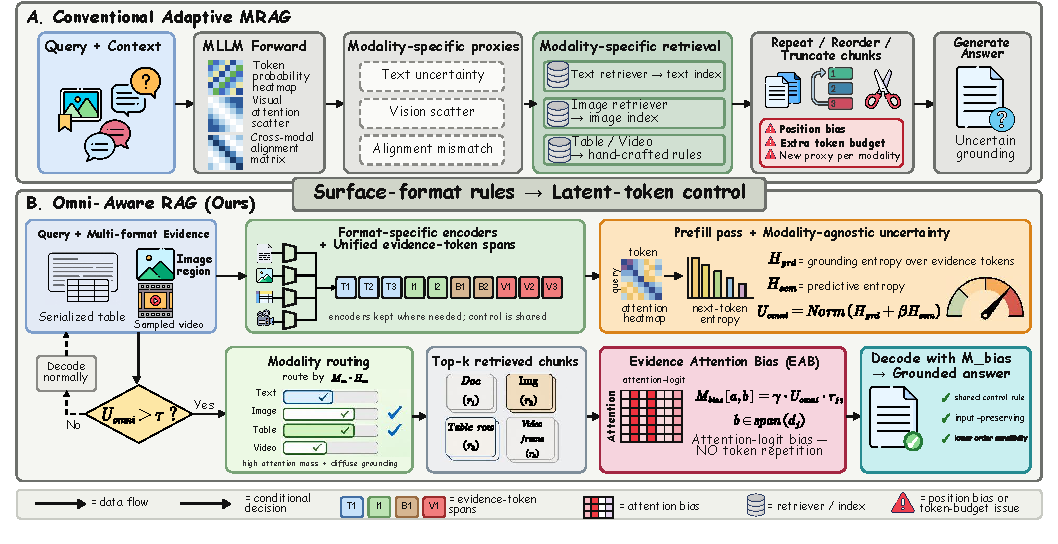
\includegraphics[width=\textwidth]{fig/fig2.pdf}
  \Description{Two-row diagram contrasting format-specific adaptive multimodal RAG pipelines with the shared span-level controller of Omni-Aware.}
  \caption{Comparison of control designs. (A) An illustrative composite of format-specific adaptive multimodal RAG designs~\cite{du2026mmarag,yeo2026universalrag,zhai2025samrag}, not a single system; each cited system uses only some of these components: each format has its own uncertainty proxy and retrieval rule, and chunks are repeated, reordered, or truncated for emphasis. (B) \method{} keeps format-specific encoders and retrievers and applies one rule to the evidence spans: $\Uomni$ gates retrieval, $M_m\cdot H_m$ routes it, and EAB biases attention toward retrieved chunks.}
  \label{fig:compare}
\end{figure*}

Retrieval selects which chunks the generator sees, whereas attention determines how much each chunk contributes to a prediction. \method{} connects the two decisions through evidence spans: every encoded chunk occupies an identifiable token span in the decoder input, while its retriever and encoder remain format-specific. The controller reads and adjusts attention over these spans and does not edit hidden activations. The same attention is read to decide and written to act. For Challenge~1, an uncertainty score from predictive entropy and the dispersion of evidence attention decides whether to retrieve, and the attention each modality receives decides which modality to search; at cold start, a probe round of retrieved chunks supplies the evidence spans that the score and the route read, so one prefill serves both decisions without a trained router. For Challenge~2, Evidence Attention Bias (EAB) adds a relevance-weighted bias to the attention logits of each retrieved chunk on every row that predicts an answer token, scaled by the uncertainty score, without duplicated input or parameter updates.

\ai{\method{} outperforms all baselines on the four benchmarks} (\ph{} versus \ph{} for M2-RAG on WebQA). Our contributions are as follows:
\begin{itemize}
  \item We identify two challenges of multimodal Web answering and measure them: formats differ in span length (\ph{} to \ph{} tokens) and score scale, and relevance-sorted and reverse-sorted orders of the same chunks differ by \ph{} points on OK-VQA.
  \item We formulate evidence acquisition and use over evidence spans and derive all three decisions from one zero-bias prefill: one uncertainty score triggers retrieval and scales chunk weighting, modality-level attention routes the retrieval, and a probe round extends both to queries without supplied context. Unlike query-only or retriever-score routers, the controller needs no training data and no sampled generations.
  \item We introduce EAB, an uncertainty-gated and relevance-weighted attention bias on the rows that predict answer tokens, including the first, and characterize its effect at a fixed attention row: it tilts chunk masses toward relevance by a bounded factor and matches chunk replication at bias $\log n$ (Propositions~\ref{thm:tilt} and~\ref{thm:dca-local}).
  \item On four benchmarks with text, image, table, and video evidence, \method{} \ai{outperforms M2-RAG, SeaKR, and UniversalRAG} and lowers the order-induced standard deviation by \ph\% to 70\%; further analyses cover routing, counterfactual evidence, and retrieval noise. All settings are fixed on development queries by rules stated before the evaluation runs (Section~\ref{sec:setup}).
\end{itemize}

%% ===============================================================
\section{Related Work}
\label{sec:related}

\textit{Web and multimodal retrieval-augmented generation.} Web answer engines retrieve and cite pages at query time~\cite{nakano2021webgpt,liu2023webglm}, and WebQA poses multimodal Web answering over text and image facts~\cite{chang2022webqa}. Multimodal RAG systems~\cite{abootorabi2025survey} retrieve images, knowledge memories, or visual documents~\cite{adjali2024multilevel,chen2022murag,hu2023reveal,wang2025vidorag,yu2025visrag}, generate multimodal answers~\cite{ma2025m2rag,wu2025visualrag}, or refine selection by reranking, reflection, or adaptive visual selection~\cite{chen2025ragvl,zhai2025samrag,zhang2024mr2ag}; they improve which chunks are retrieved and how each format is encoded. We keep such format-specific components and add control over evidence acquisition and use inside the generator.

\textit{Adaptive evidence acquisition.} Adaptive retrieval decides from the generation state whether external knowledge is needed: Self-RAG learns reflection signals~\cite{asai2024selfrag}, FLARE retrieves when upcoming tokens have low probability~\cite{jiang2023flare}, DRAGIN combines token entropy with attention to decide when and what to retrieve~\cite{su2024dragin}, Adaptive-RAG classifies question complexity~\cite{jeong2024adaptiverag}, and SeaKR measures the consistency of sampled hidden states~\cite{yao2025seakr}; their cost--quality tradeoffs have been compared~\cite{moskvoretskii2025adaptive}. For multimodal inputs, MMA-RAG classifies hidden states of the input and the retrieved visual context~\cite{du2026mmarag}, and UniversalRAG routes the query alone to modality- and granularity-specific corpora~\cite{yeo2026universalrag}; retriever signals do not reliably improve such query-only routers~\cite{li2026beyond}. These methods read generated text, the query, retriever scores, or pooled hidden states, and most train a router or classifier or sample many generations. Our controller reads how the generator attends to the evidence spans of each modality, from one prefill and without training, and reuses this signal to weight the evidence.

\textit{Inference-time evidence control.} Position sensitivity~\cite{liu2024lost} has motivated multi-scale positional encoding~\cite{zhang2024mspoe} and positional attention calibration~\cite{hsieh2024found}; text-only RAG readers are less affected than long-context models~\cite{cuconasu2025positional}, but multimodal readers strongly prefer the first passages, and reranking does not remove this preference~\cite{liu2026lostend}. OpenDecoder multiplies attention scores by retrieval features and fine-tunes the decoder~\cite{mo2026opendecoder}; PASTA emphasizes user-specified spans on profiled heads~\cite{zhang2024pasta}, which at one attention row equals a constant span bias; PAI amplifies attention to image tokens~\cite{liu2024pai}; and MAD-RAG restores attention to question-relevant image regions that retrieved text draws away~\cite{zhao2026madrag}. EAB differs in three respects: each retrieved chunk receives its own bias, set by calibrated relevance and the uncertainty score; this weighting is coupled to the retrieval decision, which the other methods take as given; and the generator stays frozen.

%% ===============================================================
\section{Problem Definition}
\label{sec:problem}

We study multimodal Web answering with retrieved evidence. An instance consists of a query $q$, optional context $c$, and an external evidence pool $\mathcal{D}=\bigcup_{m\in\mathcal{M}}\mathcal{D}_m$, where $\mathcal{M}$ contains the available text, image, table, and video modalities. The context $c$ may be empty, as in a text-only WebQA question. Each chunk $d_j\in\mathcal{D}$ is the unit that can be packed into the input and keeps its source identifier and modality. For a query, the format-specific retriever of modality $m$ returns candidate chunks with raw scores $s_j$, whose scales differ across modalities.

\textit{Input and output.} A frozen generator $G_\theta$ consumes $X=[X_{\mathrm{sys}},\allowbreak X_{\mathrm{ctx}},\allowbreak X_{\mathrm{query}}]$. Here $X_{\mathrm{sys}}$ holds the task instruction and the citation format, $X_{\mathrm{ctx}}$ the encoded context and retrieved chunks, and $X_{\mathrm{query}}$ the question. The token positions that an encoded chunk occupies in $X$ form its evidence span $\mathrm{span}(d_j)$; the supplied context also occupies evidence spans, whereas $X_{\mathrm{sys}}$ and $X_{\mathrm{query}}$ do not. The output is an answer $y$ with citations to the supplied chunks, generated autoregressively from $p(\cdot\mid X,y_{<t})$.

\textit{Control decisions.} For each query, a controller makes three decisions: (i) whether additional evidence is needed; (ii) if so, which modalities $\mathcal{M}'\subseteq\mathcal{M}$ to search, retrieving at most $k$ chunks $\{d_j\}_{j=1}^{k}$; and (iii) how strongly each retrieved chunk influences decoding. The goal is a correct answer supported by the cited chunks, with $G_\theta$ frozen and the context budget fixed.

%% ===============================================================
\section{Method}
\label{sec:method}

\subsection{Framework Overview}
\method{} controls evidence acquisition and use through evidence spans (Figure~\ref{fig:pipeline}). Format-specific encoders and retrievers produce the spans (steps 1--3). Uncertainty estimation (Section~\ref{sec:uncertainty}, step 4) decides whether more evidence is needed, modality routing (Section~\ref{sec:routing}, step 5) chooses the modalities to search, and EAB (Section~\ref{sec:eab}, step 6) reuses the uncertainty score to shift attention toward relevant retrieved chunks. The first two decisions address Challenge~1; EAB addresses Challenge~2.

The interface between the format-specific components and the controller is a span map from each encoded chunk to its evidence span and modality. Serialized tables keep header and row boundaries, and video frames keep their temporal order. Spans are not compressed; the figures show them schematically.

\begin{figure*}[t]
  \centering
  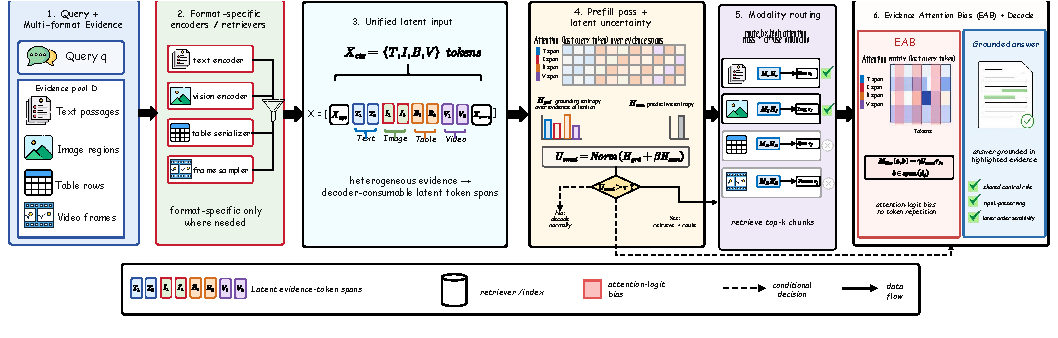
\includegraphics[width=\textwidth]{fig/fig3.pdf}
  \Description{Six-step pipeline: format-specific encoding, span map, prefill uncertainty, modality routing, and attention bias during decoding.}
  \caption{\method{} with initial multimodal context. Steps 1--3 encode the query and supplied evidence into evidence spans; step 4 computes $\hgrd$ and $\hpred$ from a zero-bias prefill (at cold start, of a probe round) and compares $\Uomni$ with $\tau$; step 5 routes retrieval by $M_mH_m$; step 6 applies EAB when $\Uomni>\taub$. In both heatmaps, columns are key positions grouped by evidence span. Rows are the attention heads of the last input position in step 4, which Eq.~\eqref{eq:attn} averages, and the rows that predict answer tokens in step 6, from the last input position on, where shaded columns receive bias.}
  %% NOTE: fig3.pdf still labels predictive entropy H_sem; re-export with H_pred
  %% and add axis labels (attention row / key position) to both heatmaps.
  \label{fig:pipeline}
\end{figure*}

\subsection{Uncertainty from Evidence and Prediction}
\label{sec:uncertainty}
To decide whether the current input suffices, the controller observes two signals: how the generator distributes attention over the available evidence, and how uncertain its next prediction is. These signals can disagree: attention can settle on one chunk while the next-token distribution remains diffuse. Both signals come from a zero-bias prefill, the forward pass over $X$ before generation.

\textit{Evidence attention.} Let $\tend$ be the last position of $X$. We read attention row $\tend$ of the final layer $L$, the row whose output predicts the first answer token, average its $n_h$ heads, and normalize over the $N$ tokens in evidence spans:
\begin{equation}
\bar A_i=\frac{1}{n_h}\sum_{h=1}^{n_h}A^{(L,h)}_{\tend,i},\qquad
A_i=\frac{\bar A_i}{\sum_{i'=1}^{N}\bar A_{i'}+\epsilon}.
\label{eq:attn}
\end{equation}
Grounding entropy measures how widely this attention is dispersed:
\begin{equation}
\hgrd=-\frac{\sum_{i=1}^{N}A_i\log(A_i+\epsilon)}{\log N},\qquad N\ge 2,
\label{eq:hgrd}
\end{equation}
and $\hgrd=0$ for $N\le1$. A high value of $\hgrd$ means that attention spreads across many evidence tokens instead of concentrating on a few. Dividing by $\log N$ bounds $\hgrd$ in $[0,1]$, though span length and image-patch density can still affect the score.

\textit{Prediction uncertainty.} Predictive entropy $\hpred$ is the normalized entropy of the next-token distribution from the same prefill,
\begin{equation}
\hpred=-\frac{\sum_{v\in\mathcal{V}}p(v\mid X)\log(p(v\mid X)+\epsilon)}{\log|\mathcal{V}|},
\label{eq:hpred}
\end{equation}
where $\mathcal{V}$ is the vocabulary.

\textit{Retrieval decision.} The uncertainty score combines the two measurements on a common scale:
\begin{align}
\Uomni&=\mathrm{Norm}(\hgrd+\beta\hpred),\label{eq:uomni}\\
\mathrm{Norm}(s)&=\mathrm{clip}\!\left(\frac{s-\mathrm{median}(S)}{1.5\,\mathrm{IQR}(S)}+0.5,\,0,\,1\right).\label{eq:norm}
\end{align}
Here $\beta$ weights predictive entropy, IQR is the interquartile range, and $S$ is the set of pre-intervention scores of unlabeled calibration queries for a given benchmark and backbone. Because $\hpred$ is small after division by $\log|\mathcal{V}|$, $\beta$ sets its share of the sum; Norm maps the median of $S$ to 0.5 so that one threshold serves all benchmarks. The controller triggers retrieval if $\Uomni>\tau$ and otherwise answers directly, retaining $\Uomni$ for the bias gate of Section~\ref{sec:eab}.

\textit{Cold start: the probe round.} When no evidence is supplied, $\hgrd=0$, and the score would reduce to normalized predictive entropy. Instead, a probe round packs the joint top-$k$ chunks over all modalities, ranked by calibrated relevance, and one zero-bias prefill of this input provides the evidence spans: $\Uomni$ is computed on them with its own calibration statistics, and the same attention gives the route of Section~\ref{sec:routing}. If $\Uomni\le\tau$, the controller answers directly and discards the probe chunks. For Web questions, a retrieval call costs little relative to generation, so the probe round trades one extra prefill for an evidence-aware decision; Section~\ref{sec:ablation} removes it.

\subsection{Modality Routing}
\label{sec:routing}
After retrieval is triggered, the controller selects the modalities to search. For modalities in the input, routing reads the attention of the same prefill, with no further forward pass. It favors modalities whose attention is substantial but diffuse. A modality with little mass barely affects the prediction, and one with concentrated attention has already located its evidence (Section~\ref{sec:ablation}).

Let $\mathcal{I}_m$ be the evidence tokens of modality $m$, pooled over all its chunks. The attention mass $M_m$ is the share of evidence attention on modality $m$, and the conditional entropy $H_m$ measures how evenly that share spreads over $\mathcal{I}_m$:
\begin{equation}
\begin{gathered}
M_m=\sum_{i\in\mathcal{I}_m}A_i,\qquad \tilde A_{m,i}=\frac{A_i}{M_m+\epsilon},\\
H_m=\frac{-\sum_{i\in\mathcal{I}_m}\tilde A_{m,i}\log(\tilde A_{m,i}+\epsilon)}{\log(\max(|\mathcal{I}_m|,2))}.
\end{gathered}
\label{eq:routing}
\end{equation}
We set $H_m=0$ when $|\mathcal{I}_m|\le1$ and select $m^\star=\arg\max_m M_mH_m$. When the two leading scores differ by at most $\delta$, both modalities are searched, and their chunks fill the $k$ slots in order of calibrated relevance $r_j$, which is comparable across modalities (Section~\ref{sec:eab}). Modalities absent from the supplied context have no attention to compare; when the supplied context covers fewer than two candidate modalities, as the query image of OK-VQA against a text corpus, routing is skipped and retrieval searches the full pool.

At cold start, the probe round of Section~\ref{sec:uncertainty} provides the evidence attention: its prefill gives $M_m\cdot H_m$ over the probe chunks, and the selected modalities are retrieved again for the final top-$k$, for instance text or image facts on WebQA. The selected retrievers return their top-$k$ chunks with scores. Routing removes nothing from the input: the supplied context remains, the retrieved chunks are packed after the supplied context and before the question, and a new prefill encodes the packed sequence and updates the span map. The $\Uomni$ of the retrieval decision is not recomputed.

\subsection{Evidence Attention Bias}
\label{sec:eab}
The attention that a packed chunk receives can vary with its position. EAB raises the influence of relevant chunks, taking as input the retrieved chunks $\{d_j\}_{j=1}^{k}$, their evidence spans, and the uncertainty score. Because raw scores $s_j$ are not comparable across modalities, per-modality percentile calibration maps each score to $r_j=\hat F_m(s_j)\in[0,1]$, where $\hat F_m$ is the empirical cumulative distribution function (ECDF) of modality-$m$ retriever scores over all retrieval candidates of the calibration queries.

With query, key, and value tensors $(Q,K,V)$, EAB adds a bias to the attention logits before the softmax:
\begin{align}
\mathrm{Attn}_{\mathrm{EAB}}&=\mathrm{softmax}\!\left(\frac{QK^\top}{\sqrt{d_k}}+M_{\mathrm{causal}}+\Mbias\right)V,\label{eq:eab}\\
\Mbias[a,b]&=\begin{cases}\gamma\,\Uomni\,r_j, & b\in\mathrm{span}(d_j),\ a\ge\tend,\\ 0, & \text{otherwise.}\end{cases}\label{eq:mbias}
\end{align}
Here $d_k$ is the key dimension, $M_{\mathrm{causal}}$ masks future positions, $a$ indexes attention rows and $b$ key positions, and $\gamma$ sets the bias strength. Only retrieved chunks receive bias; instructions, supplied context, and the question keep zero bias. The supplied context has no retriever score and thus no relevance prior, so its share of attention shrinks relative to biased chunks; Section~\ref{sec:ablation} also biases the context to test this choice. The bias acts in all decoder layers and changes neither the packed sequence nor the parameters.

\textit{Bias gate.} EAB is active on triggered queries with $\Uomni>\taub$. The second threshold $\taub\ge\tau$ reserves the bias for the most uncertain queries. With $\tau=0.35$ and $\taub=0.40$, queries with $0.35<\Uomni\le0.40$ receive evidence without bias, and biasing every triggered query lowers OK-VQA accuracy from \ph{} to \ph{} (Appendix~\ref{app:supp}). EAB is active for \ph\% of OK-VQA queries.

\textit{Prediction timing.} Row $\tend$, the last input position, predicts the first answer token at $\tans=\tend+1$, and every later row $a\ge\tans$ predicts the next one. EAB biases all of these rows. Starting at $\tans$ instead (decode-only EAB) would leave the first answer token to the unbiased prefill, and the first token alone determines most short answers, such as an entity or a number (Section~\ref{sec:setup}); Section~\ref{sec:ablation} compares the two. Biasing row $\tend$ changes only the final position of the prefill, so the key--value cache of the packed input is computed once and shared with the unbiased arm.

\textit{Effect on chunk masses.} Fix one layer, head, attention row, and visible key set, with pre-bias attention $\alpha_i$. Let $\mu_j=\sum_{i\in\mathrm{span}(d_j)}\alpha_i$ be the attention mass of chunk $j$, and let the remaining keys form a group $j=0$ with $r_0=0$. Set $\lambda=\gamma\Uomni$ when the gate is active and $\lambda=0$ otherwise.

\begin{proposition}[Bounded relevance tilt]
\label{thm:tilt}
Under EAB, the attention within each span keeps its proportions, and the chunk masses become
\begin{equation}
\mu_j'=\frac{\mu_j e^{\lambda r_j}}{\sum_{l=0}^{k}\mu_l e^{\lambda r_l}}.
\label{eq:local}
\end{equation}
For any two chunks $\mu'_j/\mu'_l=(\mu_j/\mu_l)\,e^{\lambda(r_j-r_l)}$ with $|\lambda(r_j-r_l)|\le\gamma$.
\end{proposition}

As a bounded relevance prior, EAB multiplies the odds between two chunks by at most $e^{1.2}\approx3.3$ (proof in Appendix~\ref{app:dca}): it can overturn a positional preference of up to $3.3\times$ between a relevant and an irrelevant chunk, while larger position effects persist. Since the shift $\lambda(r_j-r_l)$ is the same under every ordering, it does not by itself predict lower order sensitivity (Section~\ref{sec:order}). Chunk replication gives the same reweighting only with integer copy counts (Proposition~\ref{thm:dca-local}).

%% ===============================================================
\section{Experiments}
\label{sec:experiments}
The v2 evaluation has not been run.
Every new experimental number below is \ph{}.
Numbers copied from the root-cause report dated 13~October~2026 are marked as such.
They were computed on the previous pipeline and are not v2 results.
Exploratory outputs of \texttt{offline\_v2} are from that old pipeline, contain known bugs, and are not the main table.
The section is a measurement study, a main table, ablations, and analysis.
No cell has been filled from a v2 run.

\subsection{Experimental Setup}
\label{sec:setup}
\textit{Splits.}
WebQA calibration is at least 500 questions and the development split is 256 questions.
Both are drawn from the training split, they are disjoint, and neither is drawn from the validation split.
The test split is all 4{,}966 validation questions.
The previous statement that calibration came from the validation split, while the reported set was the entire validation split, is withdrawn.
OK-VQA uses 500 calibration questions, 256 development questions, and the remainder of the validation split as the test set.
The three OK-VQA splits are pairwise disjoint.
An empty test split is an error.
When the validation split has 5{,}046 questions, the remainder is 4{,}290.
MMQA and video are generalization settings whose sizes follow the available assets.
The current command interface does not include them, and their scores are \ph{}.

\textit{Settings and metrics.}
The primary WebQA setting is the distractor pool (\texttt{webqa\_full}), in which each question brings its own candidates.
Open retrieval (\texttt{webqa\_open\_*}; the current interface generates \texttt{webqa\_open\_img} at stage~s2) is the second setting.
OK-VQA is scored with official VQA accuracy only.
WebQA's primary metric is acc$_{\mathrm{approx}}$.
Normalized BART and QA$_{\mathrm{approx}}$ are reported as well, on the full set and on the image and text subsets.
The image subset has 2{,}511 questions and the text subset has 2{,}455.
Loose lexical WebQA scores are not placed next to acc$_{\mathrm{approx}}$.

\textit{Actions and the strong baseline.}
The decoded actions are \texttt{direct}, \texttt{static\_text}, \texttt{static\_image}, \texttt{static\_mixed}, and \texttt{rerank\_static}.
Adaptive comparators are an NTE trigger, SeaKR, the previous $\Uomni$ gate (v1), and UniversalRAG routing.
They are not eligible to be the strong baseline.
The strong baseline is the single action with the best calibration-set score.
Primary relative gain uses that score as the denominator.
The tables also report gain versus \texttt{static\_mixed}.
The oracle is the per-question best action in the same set.
Evidence Attention Bias is not a main-method arm.
All actions in a run share one prompt, one budget, and one candidate pool.
The prompt is frozen on the development split.
The test split is scored once after \texttt{docs/dev\_decisions.json} is frozen.
Grids are not selected on the test split.
The operating point previously taken from a test-set grid (Table~20 in the audited draft) is withdrawn.

\textit{Statistics.}
Uncertainty is a paired bootstrap 95\% confidence interval over questions.
Multiple comparisons use Holm correction.
Decoding is greedy, so a configuration is deterministic given its inputs.
This draft does not report a seed standard deviation under greedy decoding.
The fraction of questions on which the chosen action scores below the strong baseline is reported with the risk-control claim.
A score below \texttt{direct} is not described as better than no retrieval.

\textit{Development gates.}
Two preregistered gates are criteria, not results, and this draft does not claim that either has passed.
After the pipeline fixes, the development-set per-question oracle is compared with the strongest single action against a relative gap of 8\%.
A selector is eligible for the frozen test run when, on the development split, its relative gain over that baseline is at least 5\%, the lower end of its paired interval is positive, and its degradation rate is at most $\delta$.
The test split is not used to make those choices.

\textit{Figures withdrawn by the root-cause report.}
The following numbers are copied from the root-cause report of 13~October~2026.
They are not v2 results, and they are not written into Tables~\ref{tab:webqa}--\ref{tab:cost}.
Relative gains of +33\% on WebQA and +15\% on OK-VQA used historical cached baselines: a cached static score of 17.9 against 23.4 for static retrieval on the same 512-question batch, a gap of 5.5 points, under different prompts, budgets, and retrieval scores.
The same report withdraws a trained controller's +8.43\% and a +14.4\% chosen on a 32-question development set.
On a 256-question OK-VQA development slice, official VQA accuracy was 61.5 for direct answering, 36.3 for static retrieval, 48.1 for the gated static arm, and 36.3 for EAB.
Direct answering won 82 questions and lost 10 against static retrieval.
The per-question maximum of direct and static on that slice was 64.4, which is 2.9 points above direct answering (about +4.7\% relative).
The gated arm and EAB are both below direct answering, so the report does not call that slice an improvement over no retrieval.
On 512 WebQA questions, static retrieval scored 59.1 acc$_{\mathrm{approx}}$, 27.4 normalized BART, and 23.4 QA.
Image questions scored 63.2 acc$_{\mathrm{approx}}$ and 13.8 QA.
Text questions scored 55.0 acc$_{\mathrm{approx}}$ and 33.0 QA.
Over 2{,}560 items, a loose WebQA scorer and official acc$_{\mathrm{approx}}$ differed by 10.5 points on average (0.699 versus 0.594).
On one static OK-VQA batch, a loose scorer gave 65.8 where official VQA accuracy was about 47.9.
A greedy-decoding figure of $\pm 0.2$ is smaller than the binomial standard error of about 0.66 points on 5{,}046 OK-VQA questions, and it is not a confidence interval.
The v2 measurement that replaces these comparisons is the placeholder tables below.

\subsection{Measurement Study}
\label{sec:measure}
The measurement reserves three quantities.
The gap between the best single action and the per-question oracle is \ph{}.
Image questions and text questions are separate columns in Tables~\ref{tab:webqa} and~\ref{tab:okvqa}, and every column is \ph{}.
The size of the normalized BART factor, reported beside acc$_{\mathrm{approx}}$, is \ph{}.
A 50-question image-evidence diagnostic is specified, and its conclusion is \ph{}.
The audit's 256-question and 512-question figures above are the motive for these tables.
They are not substitutes for the cells.

\begin{table*}[t]
\caption{WebQA distractor test split (\texttt{webqa\_full}): placeholder measurement.
acc$_{\mathrm{approx}}$ is primary.
Normalized BART and QA$_{\mathrm{approx}}$ are secondary.
Image and text are subsets of the same run.
The strong baseline is whichever single action scores highest on the calibration split; its identity is frozen before test and is not chosen on this table.
The oracle is the per-question best action.
Every entry is \ph{}.
The v2 run has not been executed.}
\label{tab:webqa}
\scriptsize
\setlength{\tabcolsep}{3.5pt}
\begin{tabular}{@{}lccccccccc@{}}
\toprule
Action & \multicolumn{3}{c}{acc$_{\mathrm{approx}}$} & \multicolumn{3}{c}{norm.\ BART} & \multicolumn{3}{c}{QA$_{\mathrm{approx}}$} \\
\cmidrule(lr){2-4}\cmidrule(lr){5-7}\cmidrule(l){8-10}
 & All & Image & Text & All & Image & Text & All & Image & Text \\
\midrule
\texttt{direct} & \ph{} & \ph{} & \ph{} & \ph{} & \ph{} & \ph{} & \ph{} & \ph{} & \ph{} \\
\texttt{static\_text} & \ph{} & \ph{} & \ph{} & \ph{} & \ph{} & \ph{} & \ph{} & \ph{} & \ph{} \\
\texttt{static\_image} & \ph{} & \ph{} & \ph{} & \ph{} & \ph{} & \ph{} & \ph{} & \ph{} & \ph{} \\
\texttt{static\_mixed} & \ph{} & \ph{} & \ph{} & \ph{} & \ph{} & \ph{} & \ph{} & \ph{} & \ph{} \\
\texttt{rerank\_static} & \ph{} & \ph{} & \ph{} & \ph{} & \ph{} & \ph{} & \ph{} & \ph{} & \ph{} \\
Strong baseline & \ph{} & \ph{} & \ph{} & \ph{} & \ph{} & \ph{} & \ph{} & \ph{} & \ph{} \\
Oracle & \ph{} & \ph{} & \ph{} & \ph{} & \ph{} & \ph{} & \ph{} & \ph{} & \ph{} \\
\bottomrule
\end{tabular}
\end{table*}

\begin{table}[t]
\caption{OK-VQA test split: official VQA accuracy only.
Placeholder measurement.
The same action definitions as Table~\ref{tab:webqa}.
Every entry is \ph{}.}
\label{tab:okvqa}
\small
\begin{tabular}{@{}lc@{}}
\toprule
Action & VQA accuracy \\
\midrule
\texttt{direct} & \ph{} \\
\texttt{static\_text} & \ph{} \\
\texttt{static\_image} & \ph{} \\
\texttt{static\_mixed} & \ph{} \\
\texttt{rerank\_static} & \ph{} \\
Strong baseline & \ph{} \\
Oracle & \ph{} \\
\bottomrule
\end{tabular}
\end{table}

\subsection{Main Results}
\label{sec:main}
Table~\ref{tab:main} is the main comparison.
Relative gain versus the strong baseline is the primary column.
Gain versus \texttt{static\_mixed} is secondary.
Each gain cell is a point estimate and a paired bootstrap 95\% interval; both are \ph{}, so the cell is written \ph{} [\ph{},\,\ph{}].
Degradation is the fraction of test questions on which the chosen action scores below the strong baseline.
No row is marked significant, because no test has been run.
A filled row that sits below \texttt{direct} will not be described as better than no retrieval.

\begin{table*}[t]
\caption{Main results on the frozen test splits.
WebQA uses acc$_{\mathrm{approx}}$ in the distractor setting.
OK-VQA uses official VQA accuracy.
``Versus strong'' uses the calibration-set best single action as the denominator.
``Versus static'' uses \texttt{static\_mixed}.
Brackets are paired bootstrap 95\% intervals.
Degr.\ is the degradation rate against the strong baseline.
All entries are \ph{}.
EAB is omitted.}
\label{tab:main}
\scriptsize
\setlength{\tabcolsep}{2.4pt}
\begin{tabular}{@{}lccccccc@{}}
\toprule
Method & \multicolumn{3}{c}{WebQA acc$_{\mathrm{approx}}$} & \multicolumn{3}{c}{OK-VQA} & Degr. \\
\cmidrule(lr){2-4}\cmidrule(lr){5-7}
 & Score & vs.\ strong & vs.\ static & Score & vs.\ strong & vs.\ static & \\
\midrule
\texttt{direct} & \ph{} & \ph{} [\ph{},\,\ph{}] & \ph{} [\ph{},\,\ph{}] & \ph{} & \ph{} [\ph{},\,\ph{}] & \ph{} [\ph{},\,\ph{}] & \ph{} \\
\texttt{static\_text} & \ph{} & \ph{} [\ph{},\,\ph{}] & \ph{} [\ph{},\,\ph{}] & \ph{} & \ph{} [\ph{},\,\ph{}] & \ph{} [\ph{},\,\ph{}] & \ph{} \\
\texttt{static\_image} & \ph{} & \ph{} [\ph{},\,\ph{}] & \ph{} [\ph{},\,\ph{}] & \ph{} & \ph{} [\ph{},\,\ph{}] & \ph{} [\ph{},\,\ph{}] & \ph{} \\
\texttt{static\_mixed} & \ph{} & \ph{} [\ph{},\,\ph{}] & \ph{} [\ph{},\,\ph{}] & \ph{} & \ph{} [\ph{},\,\ph{}] & \ph{} [\ph{},\,\ph{}] & \ph{} \\
\texttt{rerank\_static} & \ph{} & \ph{} [\ph{},\,\ph{}] & \ph{} [\ph{},\,\ph{}] & \ph{} & \ph{} [\ph{},\,\ph{}] & \ph{} [\ph{},\,\ph{}] & \ph{} \\
NTE trigger & \ph{} & \ph{} [\ph{},\,\ph{}] & \ph{} [\ph{},\,\ph{}] & \ph{} & \ph{} [\ph{},\,\ph{}] & \ph{} [\ph{},\,\ph{}] & \ph{} \\
SeaKR & \ph{} & \ph{} [\ph{},\,\ph{}] & \ph{} [\ph{},\,\ph{}] & \ph{} & \ph{} [\ph{},\,\ph{}] & \ph{} [\ph{},\,\ph{}] & \ph{} \\
v1 $\Uomni$ gate & \ph{} & \ph{} [\ph{},\,\ph{}] & \ph{} [\ph{},\,\ph{}] & \ph{} & \ph{} [\ph{},\,\ph{}] & \ph{} [\ph{},\,\ph{}] & \ph{} \\
UniversalRAG & \ph{} & \ph{} [\ph{},\,\ph{}] & \ph{} [\ph{},\,\ph{}] & \ph{} & \ph{} [\ph{},\,\ph{}] & \ph{} [\ph{},\,\ph{}] & \ph{} \\
v2-Rule & \ph{} & \ph{} [\ph{},\,\ph{}] & \ph{} [\ph{},\,\ph{}] & \ph{} & \ph{} [\ph{},\,\ph{}] & \ph{} [\ph{},\,\ph{}] & \ph{} \\
v2-Cal & \ph{} & \ph{} [\ph{},\,\ph{}] & \ph{} [\ph{},\,\ph{}] & \ph{} & \ph{} [\ph{},\,\ph{}] & \ph{} [\ph{},\,\ph{}] & \ph{} \\
Oracle & \ph{} & \ph{} [\ph{},\,\ph{}] & \ph{} [\ph{},\,\ph{}] & \ph{} & \ph{} [\ph{},\,\ph{}] & \ph{} [\ph{},\,\ph{}] & \ph{} \\
\bottomrule
\end{tabular}
\end{table*}

\subsection{Ablations}
\label{sec:ablation}
Table~\ref{tab:ablation} removes one v2-Cal feature at a time, compares v2-Rule with v2-Cal, and leaves a row for the preregistered level $\alpha=\delta=0.10$.
The $\delta$ row is a development-split description.
It is not a point selected on the test set.
Refitting uses the calibration split only.
Every entry is \ph{}.

\begin{table}[t]
\caption{Ablations on the frozen test metrics after calibration-split refits.
WebQA is acc$_{\mathrm{approx}}$.
OK-VQA is official VQA accuracy.
Utility is Equation~\eqref{eq:loss} on the calibration split and is not an accuracy.
Every entry is \ph{}.
The $\delta$ row is not used to pick the test operating point.}
\label{tab:ablation}
\scriptsize
\setlength{\tabcolsep}{3pt}
\begin{tabular}{@{}lcccc@{}}
\toprule
Variant & WebQA & OK-VQA & Degr. & Utility \\
\midrule
v2-Cal, six features & \ph{} & \ph{} & \ph{} & \ph{} \\
Without normalized entropy & \ph{} & \ph{} & \ph{} & \ph{} \\
Without logit margin & \ph{} & \ph{} & \ph{} & \ph{} \\
Without sequence log-prob. & \ph{} & \ph{} & \ph{} & \ph{} \\
Without length & \ph{} & \ph{} & \ph{} & \ph{} \\
Without KL vs.\ direct & \ph{} & \ph{} & \ph{} & \ph{} \\
Without retriever gap & \ph{} & \ph{} & \ph{} & \ph{} \\
v2-Rule & \ph{} & \ph{} & \ph{} & \ph{} \\
Development $\delta=0.10$ & \ph{} & \ph{} & \ph{} & \ph{} \\
\bottomrule
\end{tabular}
\end{table}

\subsection{Open Retrieval, Generalization, and Cost}
\label{sec:extra}
Table~\ref{tab:open} is the open-retrieval image setting.
The current interface builds it with stage~s2, not with a frozen stage-s4 test, so the table is not a test result.
Generalization to MMQA and to video is \ph{} and has no command in that interface.
Table~\ref{tab:cost} reserves mean generator calls, input tokens, and latency.
Planning estimates of GPU time are not entered here.

\begin{table}[t]
\caption{Open-retrieval WebQA image setting (\texttt{webqa\_open\_img}), stage~s2 interface only.
Not a frozen test.
Primary metric acc$_{\mathrm{approx}}$, plus normalized BART and QA$_{\mathrm{approx}}$.
Every entry is \ph{}.}
\label{tab:open}
\small
\begin{tabular}{@{}lccc@{}}
\toprule
Action & acc$_{\mathrm{approx}}$ & norm.\ BART & QA$_{\mathrm{approx}}$ \\
\midrule
\texttt{direct} & \ph{} & \ph{} & \ph{} \\
\texttt{static\_text} & \ph{} & \ph{} & \ph{} \\
\texttt{static\_image} & \ph{} & \ph{} & \ph{} \\
\texttt{static\_mixed} & \ph{} & \ph{} & \ph{} \\
\texttt{rerank\_static} & \ph{} & \ph{} & \ph{} \\
\bottomrule
\end{tabular}
\end{table}

\begin{table}[t]
\caption{Cost placeholders on the stage-s4 runs.
Calls, input tokens, and latency are \ph{}.
The cheap variant decodes evidence actions only when the direct signal is below its threshold.}
\label{tab:cost}
\small
\begin{tabular}{@{}lccc@{}}
\toprule
System & Calls & Input tokens & Latency \\
\midrule
\texttt{direct} only & \ph{} & \ph{} & \ph{} \\
Always \texttt{static\_mixed} & \ph{} & \ph{} & \ph{} \\
SeaKR & \ph{} & \ph{} & \ph{} \\
v2, all actions & \ph{} & \ph{} & \ph{} \\
v2, cheap variant & \ph{} & \ph{} & \ph{} \\
\bottomrule
\end{tabular}
\end{table}

\subsection{Attention steering moves attention, not answers}
\label{sec:steer}
Every number in this subsection is copied from the root-cause report dated 13~October~2026.
The measurements come from the previous pipeline.
They are not v2 results, and they are not taken from \texttt{offline\_v2}.

On a 64-question probe, the L1 distance of attention toward the supporting block moved from 0.77 to 0.26, and the answer flipped on 2 of 64 questions.
On the 38 questions in that probe where the gate was on, the median gap between the top-1 and top-2 first-token logits was about 3.4--3.5, and the median largest logit displacement caused by the bias was about 2.0.
On 29 of those 38 questions the gap exceeded the displacement.
The two flips had gaps of 0 and 0.75.
First-token predictive entropy was about 0.01--0.02, and on 65\% of questions $h_{\mathrm{sem}}<0.01$.
Before the bias, about 59\% of the attention already lay on the supporting evidence.
The bias raised that absolute mass by 0.011 on average.
The largest bias was about 1.2 nats (median of the per-question maximum 0.78, 90th percentile 1.07).
Among 306 gated-on questions, the median attention odds between the best and worst chunk were 1.185, against the propositional upper bound $e^{1.2}=3.32$ at $U=1$ and a full relevance gap.
The same gap is why a uniform span bias in the style of PASTA, or a positional recalibration in the style of Found-in-the-Middle, has little room to change an answer the first token has already determined.
This draft does not report a new PASTA or Found-in-the-Middle run.

On 512 questions decoded under one protocol on CUDA, the first token changed on 14 questions.
EAB-P versus static retrieval changed official QA by +1.30\%, with a 95\% interval of $[-0.11,+0.87]$ points, which includes zero.
The same comparison on MPS was +1.20\% and also includes zero.
Of a +0.304 point QA difference, two questions contributed +0.195 and +0.122, and the other 510 questions summed to $-0.013$.
Replacing CUDA with MPS and adding no bias changed 62 of 512 answers.
EAB-P changed 55--64 answers.

The bias formula applies on rows $a\ge\tend$ (implementation name \texttt{ans1}).
A previous default applied the bias only on decode rows (\texttt{ans2}) and was labeled as the paper form.
That label is withdrawn.
The gate in those runs read $U_{\mathrm{post}}$, not the retrieval-time uncertainty named in the text.
Appendix~\ref{app:dca} records the local algebra of this retired bias.
It is not an accuracy result.

\subsection{Failure Cases and Format Sensitivity}
\label{sec:cases}
Failure counts for missing evidence, wrong modality, and format mismatch are \ph{}.
No case is filled in, because the v2 runs have not been executed.
Format sensitivity uses the single frozen prompt from Section~\ref{sec:setup}.
A comparison across prompt variants, if it is run, is a development-split description and is \ph{} here.
It is not a search over prompts on the test split.

%% ===============================================================
\section{Conclusion}
We describe \method{} v2, a per-question choice among direct answering, static text, static image, static mixed evidence, and reranked static evidence.
v2-Rule fits no weights.
v2-Cal is one logistic regression with seven parameters.
Fixed-sequence Learn-then-Test at $\alpha=\delta=0.10$ supplies the degradation-rate claim in Section~\ref{sec:risk}, which does not say that the method is never worse.
The primary comparison uses the strongest single action on the calibration split as the denominator.
The measurement, the main table, and the ablations have not been run, and their numbers are \ph{}.
The attention-steering subsection quotes the 13~October~2026 root-cause report: attention moves, and answers do not.
Appendix~\ref{app:limitations} states the limitations.


\bibliographystyle{ACM-Reference-Format}
\bibliography{references}

\appendix
%% ===============================================================

\section{Evaluation Details}
\label{app:protocol}
\textit{Evidence pools.} OK-VQA retrieves Wikipedia passages from the DPR corpus~\cite{karpukhin2020dpr}. WebQA retrieves from the full validation pool of text snippets and images; \webimg{} contains the image-based validation questions, whose gold facts are images; every WebQA question is posed in text, so retrieving from the full text-and-image pool tests routing from text queries to visual evidence. HybridQA and VideoRAG-Synth use the unified corpora of the UniversalRAG suite~\cite{yeo2026universalrag}: Web tables with their linked passages, and HowTo100M videos with transcripts and fixed clip segments. Their candidates are the top five per modality returned by the suite's own retrievers (text and tables with its text embedder, videos and clips with its multimodal embedder, video scores mixed with transcript scores at weight 0.2), exported once and shared by every method. On average, a text chunk occupies \ph{} decoder tokens, a serialized table \ph, an image \ph, and a video chunk \ph; raw retriever scores range from \ph{} to \ph{} for text and from \ph{} to \ph{} for images. Within the top-$k$, the calibrated relevance $r_j$ of the first and the fifth chunk differs by \ph{} on average. In component ablations, static concatenation and EAB use the same packed sequence, whereas chunk replication duplicates those chunks before truncation under the same input budget. Our controller rescores these candidates: a video or clip receives the mean of the per-modality percentiles of its transcript BGE score and of the CLIP score of its mean frame embedding.

\textit{Cold-start routing and incremental decoding.} At cold start, routing runs after the trigger: the joint top-$k$ round is packed without bias, one prefill gives $M_m\cdot H_m$ over its evidence spans, and only the final top-$k$ inside the routed modalities is used for answering; the first-round chunks are not reused. During incremental decoding, the biases assigned to evidence keys are kept across steps.

\textit{Implementation.} EAB is an additive mask of shape $[\mathrm{batch},1,q_{\mathrm{len}},kv_{\mathrm{len}}]$ that broadcasts across heads and grows along the key dimension as positions enter the key--value (KV) cache. Attention and entropy computations use $\epsilon=10^{-9}$. The strength $\gamma$ is chosen from $\{0.6,0.9,1.2,1.5,2.0\}$ on development queries, and applying EAB to all decoder layers outperforms applying it to the last four by 0.6 points. Decoding uses eager or scaled dot-product attention, since FlashAttention-2 may ignore non-binary masks.

\textit{Calibration protocol.} Each calibration query stores $\hgrd+\beta\hpred$ computed before any intervention, together with the raw scores of its retrieval candidates per modality. Probe-round scores of cold-start calibration queries form a separate set $S$ with its own median and IQR. The median, IQR, and per-modality ECDFs are then frozen for all evaluation runs; when $\mathrm{IQR}(S)=0$, it is floored at $10^{-6}$.

\textit{Development grid and decision rules.} The development runs compare six EAB forms (start row $\tend$, $\tans$, or the first question token, times bias $\gamma\Uomni r_j$ or $\gamma\Uomni(2r_j-1)$), three uncertainty variants (the sum of Eq.~\eqref{eq:uomni}; the same sum after standardizing $\hgrd$ and $\hpred$ separately by their calibration median and IQR; and the attention of the middle decoder layer instead of the last), and three OK-VQA corpora (BM25 and BGE over Wikipedia passages of DPR~\cite{karpukhin2020dpr}, and BGE over GS-112K). One EAB form is chosen for all benchmarks: the one with the largest same-input gain over static concatenation, averaged over benchmarks with equal weight; it counts as effective only if the stratified bootstrap 95\% interval of this gain excludes zero. The uncertainty variant maximizes the mean Spearman correlation between the score and the error of direct answers. The OK-VQA corpus maximizes the gain of static concatenation over direct answering. Selected: \tbd{[[EAB form, uncertainty variant, corpus; fill from runs/dev\_decisions.json]]}.

\textit{Citation support.} Every chunk carries a normalized identifier such as \texttt{[E3]}. Missing, malformed, and out-of-prompt citations receive zero credit, and Inv.\ is the share of citation markers that are malformed (any identifier not of the form \texttt{[E$j$]}) or point outside the prompt, among all citation markers. For answer $y$ to question $x$, cited chunks $C(x)$, and a binary support checker $\mathcal{S}$, let $\mathrm{Supp}(x)=\sum_{e\in C(x)}\mathcal{S}(y,e)$. Faith is $\mathbb{I}[\mathrm{Supp}(x)>0]$, and attribution precision is $\mathrm{Supp}(x)/|C(x)|$. Faith is averaged over all answers and attribution precision over the answers with at least one citation, which make up \ph\% of OK-VQA answers; hence coverage times attribution precision cannot exceed Faith. Support checking first applies alias matching, which accepts a cited chunk when a gold alias occurs both in the answer statement that cites it and in the chunk, and otherwise sentence-level NLI with DeBERTa-v3-large (MoritzLaurer/DeBERTa-v3-large-mnli-fever-anli-ling-wanli, revision b3546ea): the chunk supports the answer when it entails an answer sentence citing it, i.e., when the entailment logit is the largest.

\textit{Attention--relevance divergence.} ARD compares the normalized attention mass $p$ of the chunks with a relevance target:
\begin{equation}
\pi_j^{\mathrm{rel}}=\frac{e^{r_j/T_r}}{\sum_l e^{r_l/T_r}},\qquad
\mathrm{ARD}=\mathrm{JSD}(p\,\|\,\pi^{\mathrm{rel}}),
\label{eq:ard}
\end{equation}
where $T_r=0.1$ is a temperature. ARD shares EAB's retriever scores, so it measures alignment with the intervention signal.

\textit{Order and routing metrics.} The orderings $\pi_1,\dots,\pi_{12}$ permute the five retrieval ranks and are applied identically to all questions. The flip indicator of question $x$ is $1$ if answer correctness differs between any two orderings, and the flip rate averages this indicator over questions. Among triggered queries with annotated gold modalities $\mathcal{M}^\ast$ and searched modalities $\mathcal{M}'$, WR is the share with $\mathcal{M}'\cap\mathcal{M}^\ast=\emptyset$ and Cov.\ the share with $\mathcal{M}^\ast\subseteq\mathcal{M}'$.

\textit{Evidence interventions.} Interventions use the queries for which retrieval triggers, EAB is active ($\Uomni>\taub$), and the gold answer string occurs in a retrieved text chunk; the highest-ranked such chunk is the target chunk, and \ph{} of the \webimg{} questions remain after these filters. The retrieval decision and the $\Uomni$ used by EAB stay those of the unperturbed run. Masking replaces every token of the target chunk by padding and keeps span positions unchanged. Counterfactual edits replace every occurrence of the gold answer in the target chunk with a same-type entity, the gold answer of another evaluation question chosen by a hash of the question identifier; types are year, number, color, yes/no, the named-entity label of spaCy \texttt{en\_core\_web\_sm}, or otherwise the word count. An answer follows the edit when it contains that entity after answer normalization. As controls, a random edit replaces a word-aligned non-answer span of the answer's length with the same entity, and an unedited rerun measures the base rate of answer changes. Distractors, the two highest-scoring candidates beyond the top $k$ that neither contain the gold answer nor are gold facts, replace the two lowest-ranked non-target chunks at their positions. Only text chunks are edited.

\textit{Retrieval errors.} Gold@2--5 contains \webimg{} questions whose top-ranked chunk is not a gold fact while a gold fact appears at ranks 2--5. Noise is added to calibrated relevance and clipped to $[0,1]$, averaged over three draws. For injection, a passage resembling a relevant Web page, with a wrong answer or an instruction to the model, replaces the lowest-ranked non-gold chunk and receives relevance $r=1$, which places it first under relevance-sorted packing; the wrong answer is the counterfactual entity above, and an answer is misled when it contains it.

%% ===============================================================
\section{Proofs for Evidence Attention Bias}
\label{app:dca}
Both propositions fix one layer, head, and attention row $a$ with pre-bias logits $s_i$ (including existing masks) and values $v_i$. Chunk $j\in\{1,\dots,k\}$ occupies evidence span $\mathrm{span}(d_j)$; the remaining visible keys form group $0$ with relevance $r_0=0$.

\textit{Proof of Proposition~\ref{thm:tilt}.} Under EAB, a key $i$ in $\mathrm{span}(d_j)$ receives logit $s_i+\lambda r_j$, so its weight is $\alpha_ie^{\lambda r_j}/\sum_{i'}\alpha_{i'}e^{\lambda r(i')}$. Because all keys in the span share $e^{\lambda r_j}$, proportions within the span are preserved; summing over the span gives Eq.~\eqref{eq:local} with $Z(\lambda)=\sum_l\mu_le^{\lambda r_l}$. For any distribution $p$ over the groups, substituting $\log\mu'_j=\log\mu_j+\lambda r_j-\log Z(\lambda)$ gives
\[
\lambda\textstyle\sum_jp_jr_j-D_{\mathrm{KL}}(p\,\|\,\mu)=\log Z(\lambda)-D_{\mathrm{KL}}(p\,\|\,\mu'),
\]
which is maximized uniquely at $p=\mu'$. The odds ratio follows by dividing two instances of Eq.~\eqref{eq:local}, and $|\lambda(r_j-r_l)|\le\gamma$ because $\lambda\le\gamma\Uomni\le\gamma$ and $r\in[0,1]$. $\square$

\textit{Relation to chunk replication.} Let chunk $j$ have $n_j$ copies, with $n_0=1$, and let EAB add $b_j$ to each logit in its span. Chunk replication (superscript $\mathrm{rep}$) repeats the key and value rows of the span. Local equivalence requires (A1) unchanged replica logits at row $a$, (A2) unchanged values, and (A3) all copies visible to row $a$.

\begin{proposition}[Local equivalence of chunk replication and EAB]
\label{thm:dca-local}
Under (A1)--(A3), pooling the weights of the copies of key $i\in\mathrm{span}(d_j)$ gives
$\tilde\alpha_i^{\mathrm{rep}}:=\sum_{\ell=1}^{n_j}\alpha^{\mathrm{rep}}_{i,\ell}=\alpha_i^{\mathrm{EAB}}\big|_{b_j=\log n_j}$,
and every key of group $0$ has the same weight under both. The chunk masses satisfy $\mu_j^{\mathrm{rep}}=\mu_j^{\mathrm{EAB}}=n_j\sum_{i\in\mathrm{span}(d_j)}e^{s_i}/D$ with
\begin{equation}
D=\sum_{i\in\text{group }0}e^{s_i}+\sum_{\ell=1}^{k}n_\ell\sum_{i\in\mathrm{span}(d_\ell)}e^{s_i},
\label{eq:dca-norm}
\end{equation}
and the attention outputs at row $a$ coincide.
\end{proposition}

\begin{proof}
By (A1) and (A3), both normalizers equal $D$ because $n_je^{s_i}=e^{s_i+\log n_j}$. Pooling the copies gives $\tilde\alpha_i^{\mathrm{rep}}=n_je^{s_i}/D=\alpha_i^{\mathrm{EAB}}\big|_{b_j=\log n_j}$, and summing within the span proves mass equality. By (A2), equal pooled weights give identical attention outputs.
\end{proof}

\textit{Boundary conditions.} Rotary position embeddings (RoPE) and the surrounding sequence can violate (A1) and (A2). Under causal attention, (A3) requires the copies to precede row $a$; with $c_j(a)>0$ visible copies, the effective bias is $\log c_j(a)$. Cross-layer residual updates can also break the matching of replica keys and values, so the full-system difference between chunk replication and EAB (\ph{} against \ph{} on OK-VQA) lies beyond this local relation.

%% ===============================================================
\section{Supplementary Results}
\label{app:supp}

\textit{Entropy weight and intervention threshold.} The values of $\beta$ and $\taub$ were selected on development queries; we report their sensitivity on the evaluation sets. Over $\beta\in\{0,0.15,0.30,0.50,1.00\}$ and $\taub\in\{0.20,0.40,0.60\}$, \ai{$\beta=0.30$ scores highest at every $\taub$ on OK-VQA}, and the selected pair ($\beta=0.30$, $\taub=0.40$) reaches \ph{} on OK-VQA and \ph{} on HybridQA. For $\beta$ between 0.15 and 0.50, OK-VQA stays between \ph{} and \ph{} and HybridQA between \ph{} and \ph. Grounding entropy alone ($\beta=0$) gives \ph{} to \ph{} on OK-VQA, and $\beta=1$ gives \ph{} to \ph. Setting $\taub=0.20<\tau$, which biases every retrieved query, gives \ph{} on OK-VQA and \ph{} on HybridQA at $\beta=0.30$.

\textit{Calibration transfer and size.} With 100 and 500 unlabeled calibration queries, OK-VQA reaches \ph{} and \ph; reusing the OK-VQA statistics on \webimg{} gives \ph{} instead of \ph, and with per-backbone statistics the controller improves both backbones on \ph{} of the four benchmarks. Reusing the OK-VQA statistics changes HybridQA from \ph{} to \ph, VideoRAG-Synth from \ph{} to \ph, and \webimg{} from \ph{} to \ph, and their retrieval rates from \ph\%, \ph\%, and \ph\% to \ph\%, \ph\%, and \ph\%. On OK-VQA, 100, 500, and 1{,}000 calibration queries give \ph{}, \ph{}, and \ph{} at retrieval rates of \ph{}\%, \ph{}\%, and \ph{}\%, so 100 queries recover \ph\% of the gain that 500 queries achieve over static concatenation. Without calibration, the controller uses heuristic default statistics, retrieves for every query, and reaches \ph{}; \tbd{[[is EAB active?]]}.

\textit{Citation support.} With the DeBERTa-v3-large checker, Faith rises from \ph{} to \ph{} on OK-VQA, from \ph{} to \ph{} on HybridQA, and from \ph{} to \ph{} on \webimg{}. Attribution precision rises from \ph{} to \ph{} on HybridQA (OK-VQA and \webimg{} in Table~\ref{tab:uomni_ablation}), and invalid citations fall from \ph{}\%, \ph\%, and \ph\% to \ph{}\%, \ph\%, and \ph\%.

\textit{Selective risk.} Scoring each system on its own answers, AURC and the Spearman $\rho$ between uncertainty and error are \ph{} and \ph{} for \method{} on \webimg{}, against \ph{} and \ph{} for SeaKR and \ph{} and \ph{} for NTE; on OK-VQA they are \ph{} and \ph{}, \ph{} and \ph{}, and \ph{} and \ph{}. AURC mixes answer quality with error ranking.

\textit{Retrieval threshold.} With chunk replication as the evidence-use operation on OK-VQA, varying $\tau$ to lower retrieval from 100\% to \ph{}\% raises accuracy to \ph{} and attribution precision to \ph{}; accuracy stays near \ph{} down to about \ph\% retrieval.

\textit{Backbone transfer.} With per-backbone calibration statistics, the controller changes the scores of InternVL3.5-8B on WebQA, OK-VQA, HybridQA, and VideoRAG-Synth from \ph, \ph, \ph, and \ph{} under static concatenation to \ph, \ph, \ph, and \ph. The EAB hook is the same additive attention mask; InternVL3.5 places its image tokens in the decoder sequence, so the span map applies unchanged. On OK-VQA, the order standard deviation of InternVL3.5-8B is \ph{} for static concatenation, \ph{} for chunk replication, and \ph{} for EAB.

\textit{Secondary metrics.} HybridQA F1 is \ph{} for static concatenation and \ph{} for \method{}; VideoRAG-Synth BERTScore is \ph{} and \ph.

\begin{table}[t]
\caption{Order sensitivity with seed deviations (12 permutations drawn with 3 seeds; deviations across the seeds' groups of four; Qwen3-VL-8B). Gap is the relevance-sorted minus reverse-sorted score; ARD measures attention--relevance alignment.}
\label{tab:order_full}
\footnotesize
\setlength{\tabcolsep}{3pt}
\begin{tabular}{@{}lcccc@{}}
\toprule
Method & Std.$\downarrow$ & Gap$\downarrow$ & Flip\%$\downarrow$ & ARD$\downarrow$\\
\midrule
\multicolumn{5}{@{}l}{\textit{OK-VQA}}\\
Static concatenation & \ph{}$\pm$\ph{} & \ph{}$\pm$\ph{} & \ph & \ph{}\\
Chunk replication & \ph{}$\pm$\ph{} & \ph{}$\pm$\ph{} & \ph & \ph{}\\
EAB (ours) & \textbf{\ph} & \textbf{\ph} & \ph & \textbf{\ph}\\
\midrule
\multicolumn{5}{@{}l}{\textit{\webimg{}}}\\
Static concatenation & \ph & \ph & \ph & \ph\\
Chunk replication & \ph & \ph & \ph & \ph\\
EAB (ours) & \ph & \ph & \ph & \ph\\
\midrule
\multicolumn{5}{@{}l}{\textit{HybridQA}}\\
Static concatenation & \ph & \ph & \ph & \ph\\
Chunk replication & \ph & \ph & \ph & \ph\\
EAB (ours) & \ph & \ph & \ph & \ph\\
\midrule
\multicolumn{5}{@{}l}{\textit{VideoRAG-Synth}}\\
Static concatenation & \ph & \ph & \ph & \ph\\
Chunk replication & \ph & \ph & \ph & \ph\\
EAB (ours) & \ph & \ph & \ph & \ph\\
\bottomrule
\end{tabular}
\end{table}

\textit{Normalizing cross-modal retrieval scores.} Per-query min--max normalization of retriever scores gives \ph{} on OK-VQA and \ph{} on \webimg{} (ARD \ph), between raw scores (\ph{}, \ph; \ph) and per-modality percentiles (\ph{}, \ph; \ph{}).

\textit{Trigger agreement.} On OK-VQA, NTE and $\Uomni$ both retrieve on \ph{}\% of queries and both skip on \ph{}\%; NTE alone retrieves on \ph{}\% and $\Uomni$ alone on \ph{}\%. Questions answered without retrieval reach \ph{} under NTE and \ph{} under $\Uomni$, while retrieved questions reach \ph{} and \ph{} in the respective complete configurations.

%% ===============================================================
\section{Public WebQA Scoring Diagnostics}
\label{app:webqa_scoring}
\textit{Public metric.} The published WebQA evaluator~\cite{chang2022webqa} computes $\mathrm{acc}_{\mathrm{approx}}$ from category-specific F1 for color, shape, number, and yes/no questions and from recall for the other categories. We combine this accuracy component $a_i$ with the ParaBank2 BARTScore checkpoint of the WebQA authors. For reference $r_i$, answer $y_i$, and reference-to-answer log score $s$,
\begin{equation}
F_i=\min\bigl\{e^{s(r_i,y_i)-s(r_i,r_i)},1\bigr\},\qquad \mathrm{QA}_{\mathrm{approx}}=\frac{100}{N}\sum_{i=1}^{N}a_iF_i.
\label{eq:webqa}
\end{equation}
Public validation has full reference answers but not the keyword labels of the hidden test set, hence the name $\mathrm{QA}_{\mathrm{approx}}$. BART scoring uses CPU FP32, eager attention, and one checkpoint for every arm.

%% ===============================================================
\section{Error and Case Analysis}
\label{app:error}
\textit{Residual errors.} Over \tbd{[[sample size and sampling]]}, categorized errors on OK-VQA and WebQA come from missing top-$k$ evidence (\ph{}\% and \ph{}\%), ambiguous visual grounding (\ph{}\% and \ph{}\%), answer normalization (\ph{}\% and \ph{}\%), and unsupported citations (\ph{}\% and \ph{}\%).

\textit{Error sources.} Missing top-$k$ evidence causes \ph{}\% of categorized errors on OK-VQA and \ph{}\% on WebQA. A reranker can recover gold evidence in the candidate pool but outside the top $k$ (recall \ph\% against \ph\% at $k=5$), \ai{consistent with the gain of adding it to the controller (Table~\ref{tab:main}).} Relative to static concatenation at the same retrieval decision, EAB turns \ph\% of OK-VQA answers from wrong to correct and \ph\% from correct to wrong. \ai{Most losses trace back to relevance errors:} \ph\% amplify a highly scored chunk without the answer, \ph\% an unrelated image region, and \ph\% a misaligned table cell.

\textit{Cases where EAB changes the answer.} In one OK-VQA example, EAB corrects the answer: \tbd{[[question; top chunk, i.e., the chunk with the largest bias; static $\to$ EAB answers]]}. In another, it amplifies a highly scored chunk without the answer, a failure category above: \tbd{[[question; top chunk; static $\to$ EAB answers]]}.

%% ===============================================================
\section{Limitations and Ethical Considerations}
\label{app:limitations}
\textit{Limitations.} \method{} needs a decoder that exposes attention and next-token probabilities. Without attention access, chunk replication gives the same reweighting with integer copy counts (Proposition~\ref{thm:dca-local}). The span interface assumes that visual tokens enter the decoder sequence; models that feed images through cross-attention layers, such as Llama-3.2-Vision, fall outside it. Grounding entropy ignores total evidence attention, can mix heads that attend to different chunks, and depends on tokenization and patch density. The probe round costs one prefill and one retrieval call per cold-start query, also when the controller then answers directly. As a bounded prior on chunk mass, EAB lowers dataset-level order sensitivity but does not make each answer order-invariant. Per-modality percentiles align score ranks across retrievers, not the probability that a chunk supports the answer. Normalization statistics are estimated per benchmark and backbone. Each retrieved video is represented by eight sampled frames and its transcript; long videos that need temporal reasoning across many frames remain untested.

\label{app:ethics}\textit{Ethical considerations.} EAB increases the influence of highly scored chunks, so low-quality, biased, adversarial, or model-directed Web content can mislead answers (Section~\ref{sec:noise}), with greater risk in medical, legal, and educational use. Source-quality filtering and prompt-injection detection before packing, reporting $\Uomni$ and the cited sources, and abstaining when $\Uomni$ stays high reduce this risk. All datasets are public; deployments on private content need access controls. \tbd{[[AI-use disclosure]]}


\end{document}
